% Part: sets-functions-relations
% Chapter: relations
% Section: trees

\documentclass[../../../include/open-logic-section]{subfiles}

\begin{document}

\olfileid{sfr}{rel}{tre}
\olsection{Bomen}

Een \emph{boom} is een bijzonder soort partiële ordening die in alle
deelgebieden van de logica een belangrijke rol speelt. Eindige bomen
komen voor in elementaire onderdelen van de logica: zo kunnen
!!{formula}s worden begrepen aan de hand van hun ontleding in een
syntaxisboom, terwijl !!{derivation}s in veel systemen voor
!!{derivation}s eveneens de vorm van eindige bomen hebben.
%
Oneindige bomen komen al voor in bewijzen van de
volledigheidsstellingen voor de propositie- en eerste-ordelogica en
worden in de hele wiskundige logica gebruikt.

Het begrip boom uit de verzamelingenleer hangt nauw samen met het
begrip boom uit de grafentheorie. Hieronder staat een afbeelding van
een (eindige) boom:

\begin{center}
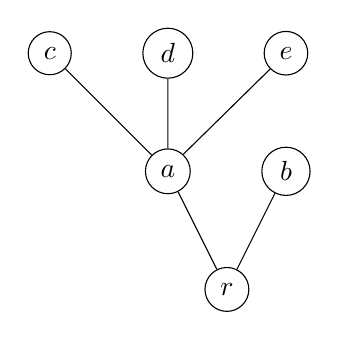
\begin{tikzpicture}[nodes={draw, circle}, -]
\node{$r$} [grow'=up]
    child { node {$a$} 
        child { node {$c$} }
        child { node {$d$} }
        child { node {$e$} }
    }
    child { node {$b$} };
\end{tikzpicture}
\end{center}

De onderste knoop~$r$ is de wortel. Elke knoop behalve $r$ heeft vlak
eronder precies één ouder. Voor knopen~$x$ en~$y$ geldt: als $y$
vanuit~$x$ kan worden bereikt door de lijnen omhoog te volgen, dan
noemen we $x$ een \emph{voorouder} van~$y$.

De voorouderrelatie in een boom is een strikte partiële ordening. Dit
vormt de aanleiding voor de definitie in termen van verzamelingen.
Daarvoor zijn twee begrippen nodig. Een \emph{kleinste element} in een
verzameling~$A$ die partieel is geordend door~$\le$, is !!a{element}
$x \in A$ waarvoor bij alle $y \in A$ geldt dat~$x \le y$. Een
verzameling heet door~$\le$ \emph{welgeordend} als iedere niet-lege
deelverzameling een kleinste element heeft.

\begin{defn}[Boom]
Een \emph{boom} is een paar $T = \tuple{A, \le}$ waarvoor $A$ een
verzameling is en $\le$ een partiële ordening op~$A$ is met precies één
kleinste element $r \in A$ (de \emph{wortel}), en waarvoor voor alle
$x \in A$ de verzameling $\Setabs{y}{y \le x}$ door~$\le$
welgeordend is.
\end{defn}

\begin{defn}[Opvolgers]
Stel dat $T = \tuple{A, \le}$ een boom is.
Als $x,y \in A$, $x < y$, en er geen $z \in A$ bestaat waarvoor
$x < z < y$, dan noemen we $y$ een \emph{opvolger} van~$x$.
\end{defn}

De opvolgers van $x \in A$ heten ook zijn \emph{kinderen}. Als $y$
een opvolger van~$x$ is, noemen we $x$ de \emph{voorganger} of
\emph{ouder} van~$y$.

\begin{prop}
Als $\tuple{A,\le}$ een boom is, heeft elk $x \in A$ behalve de wortel
hoogstens één voorganger.
\end{prop}

\begin{proof}
  Stel dat $y_1 < x$ en $y_2 < x$ en dat $y_1 \neq y_2$. Dan geldt
  $\{y_1, y_2\} \subseteq \Setabs{z}{z<x}$. Omdat
  $\Setabs{z}{z<x}$ door~$\le$ welgeordend is, heeft de deelverzameling
  $\{y_1, y_2\}$ een kleinste element, dat uiteraard $y_1$ of~$y_2$
  moet zijn. Dus $y_1 \le y_2$ of $y_2 \le y_1$. We hebben
  $y_1 \neq y_2$ aangenomen, zodat zelfs $y_1 < y_2$ of $y_2 < y_1$
  geldt. Omdat we ook $y_1 < x$ en $y_2 < x$ hebben aangenomen, geldt
  bovendien $y_1 < y_2 < x$ of $y_2 < y_1 < x$. De elementen $y_1$
  en $y_2$ kunnen dus niet beide voorgangers van~$x$ zijn.
\end{proof}

\begin{defn}
Een boom $T = \tuple{A, \le}$ heet \emph{oneindig} als $A$ een
oneindige verzameling is, en anders \emph{eindig}. Als voor $T$ geldt
dat elke $x \in A$ slechts eindig veel opvolgers heeft, heet $T$ \emph{eindig
vertakkend}.
\end{defn}

\begin{defn}[Takken]
Zij $T = \tuple{A, \le}$ een boom. Een \emph{tak} van~$T$ is een
maximale keten in~$T$, d.w.z. een verzameling $B \subseteq A$ waarvoor
voor alle $x, y \in B$ geldt dat $x \le y$ of $y \le x$, en waarvoor
voor elke $z \in A \setminus B$ een $u \in B$ bestaat zodat noch
$z \le u$ noch $u \le z$ geldt.
%
Met $[T]$ duiden we de verzameling van alle takken van $T$ aan.
\end{defn}

\begin{ex}
Een klassiek voorbeeld van een eindig vertakkende boom is de
\emph{oneindige binaire boom} van eindige rijen van $0$'en en~$1$'en.
Deze wordt soms aangeduid met $\{0,1\}^*$ of~$\Bin^*$ en is geordend
door de uitbreidingsrelatie $\sqsubseteq$ (bijv.
$101 \sqsubseteq 101101$). Omdat iedere binaire rij steeds kan worden
uitgebreid door achteraan een $0$ of een $1$ toe te voegen, bevat deze
boom oneindig veel elementen: elk element~$s$ heeft precies twee
opvolgers, $s0$ en~$s1$. De wortel is de lege rij $\emptyseq$.
\end{ex}

\begin{ex}
Iets algemener is ook de verzameling van eindige rijen van natuurlijke
getallen~$\Nat^*$ met de uitbreidingsrelatie~$\sqsubseteq$ een boom.
Deze is duidelijk niet eindig vertakkend: elke $s \in \Nat^*$ heeft
oneindig veel opvolgers~$sn$, één voor elke $n \in \Nat$. Elke
$A \subseteq \Nat^*$ die onder~$\sqsubseteq$ gesloten is, is een
\emph{deelboom} van~$\Nat^*$. (Dat wil zeggen: $A$ is zo dat uit
$s \in A$ en $s' \sqsubseteq s$ ook $s' \in A$ volgt.) Alle eindige
bomen kunnen worden weergegeven als eindige deelbomen van~$\Nat^*$.
\end{ex}

\begin{prop}[Lemma van K\H{o}nig]
Als $T = \tuple{A,\le}$ een eindig vertakkende oneindige boom is, dan
heeft $T$ een oneindige tak.
\end{prop}

In de berekenbaarheidstheorie gebruikt men vaak een speciaal geval van
het lemma van K\H{o}nig. Dit staat bekend als het \emph{zwakke lemma van
K\H{o}nig}: elke oneindige deelboom van $\{0,1\}^*$ heeft een
oneindige tak.
\end{document}
